\subsubsection{Benchmarks for operator splitting}
\label{sec:benchmark-operator_splitting}

\textit{This section was contributed by Juliane Dannberg.}

Models of mantle convection and lithosphere dynamics often also contain reactions between materials with different chemical compositions, or processes that can be described as reactions.
The most common example is mantle melting: When mantle temperatures exceed the solidus, rocks start to melt. As this is only partial melting, and rocks are a mixture of different minerals, which all contain different chemical components, melting is not only a phase transition, but also leads to reactions between solid and molten rock. Some components are more compatible with the mineral structure, and preferentially stay in the solid rock, other components will mainly move into the mantle melt. This means that the composition of both solid and melt change over time depending on the melt fraction.

Usually, it is assumed that these reactions are much faster than convection in the mantle. In other words, these reactions are so fast that melt is assumed to be always in equilibrium with the surrounding solid rock. In some cases, the formation of new oceanic crust, which is also caused by partial melting, is approximated by a conversion from an average, peridotitic mantle composition to mid-ocean ridge basalt, forming the crust, and harzburgitic lithosphere, once material reaches a given depth. This process can also be considered as a reaction between different compositional fields.

This can cause accuracy problems in geodynamic simulations: The way the equations are formulated (see Equations~\ref{eq:stokes-1}--\ref{eq:compositional}), ideally we would need to know reaction rates (the $q_i$) between the different components instead of the equilibrium value (which would then have to be compared with some sort of ``old solution'' of the compositional fields). Sometimes we also may not know the equilibrium, and would only be able to find it iteratively, starting from the current composition. In addition, the reaction rate for a given compositional field usually depends on the value of the field itself, but can also depend on other compositional fields or the temperature and pressure, and the dependence can be nonlinear.

Hence, \aspect{} has the option to decouple the advection from reactions between compositional fields, using operator splitting.

Instead of solving the coupled equation
\begin{align}
  \frac{\partial \mathfrak{c}(t)}{\partial t} + \mathbf u\cdot\nabla \mathfrak{c}(t)
  &=
  q(\mathfrak{c}(t)),
\end{align}
and directly obtaining the composition value $\mathfrak{c}(t^{n+1})$ for the time step $n+1$ from the value $\mathfrak{c}(t^{n})$ from the previous time step $n$, we do a first-order operator split, first solving the advection problem
\begin{align}
  \frac{\partial \mathfrak{c}(t)}{\partial t} + \mathbf u\cdot\nabla \mathfrak{c}(t)
  &=
  0,
  &
  \text{obtaining } \Delta \mathfrak{c}_A(t^{n+1}) \text{ from } \mathfrak{c}(t^{n}),
\end{align}
using the advection time step $\Delta t_A = t^{n+1} - t^{n}$.
Then we solve the reactions as a series of coupled ordinary differential equations
\begin{align}
  \frac{\partial \Delta \mathfrak{c}_R(t)}{\partial t}
  &=
  q(\mathfrak{c}(t^n))+\Delta \mathfrak{c}_A(t^{n+1})+\Delta \mathfrak{c}_R(t),
  &
  \text{obtaining } \Delta \mathfrak{c}_R(t^{n+1}) \text{ from } \mathfrak{c}(t^n)+\Delta \mathfrak{c}_A(t^{n+1}).
\end{align}
This can be done in several iterations, choosing a different, smaller time step size $\Delta t_R \leq \Delta t_A$ for the time discretization.
The updated value of the compositional field after the overall (advection + reaction) time step is then obtained as
\begin{align}
  \mathfrak{c}(t^{n+1})
  &=
  \mathfrak{c}(t^{n}) + \Delta \mathfrak{c}_A(t^{n+1})+\Delta \mathfrak{c}_R(t^{n+1}).
\end{align}

This is very useful if the time scales of reactions are different from the time scales of convection.
The same scheme can also be used for the temperature: If we want to model latent heat of melting, the temperature evolution is controlled by the melting rate, and hence the temperature changes on the same time scale as the reactions.

We here illustrate the way this operator splitting works using the simple example of exponential decay in a stationary advection field. We will start with a model that has a constant initial temperature and composition and no advection. The reactions for exponential decay
\begin{align}
  \mathfrak{c}(t)
  &=
  \mathfrak{c}_0 e^{\lambda t} \text{ with } \lambda = - \log(2)/t_{1/2},
\end{align}
where $\mathfrak{c}_0$ is the initial composition and $t_{1/2}$ is the half life, are implemented in a shared library
(\url{benchmarks/operator_splitting/exponential_decay/exponential_decay.cc}).
As we split the time-stepping of advection and reactions, there are now two different time steps in the model:
We control the advection time step using the `Maximum time step' parameter (as the velocity is essentially 0,
we can not use the CFL number), and we set the reaction time step using the `Reaction time step' parameter.
\lstinputlisting[language=prmfile]{cookbooks/benchmarks/operator_splitting/doc/exponential_decay.part.1.prm.out}
To illustrate convergence, we will vary both parameters in different model runs.

In our example, we choose $\mathfrak{c}_0=1$, and specify this as initial condition using the \texttt{function} plugin for both composition and temperature. We also set $t_{1/2}=10$, which is implemented as a parameter in the \texttt{exponential decay} material model and the \texttt{exponential decay heating} model.
\lstinputlisting[language=prmfile]{cookbooks/benchmarks/operator_splitting/doc/exponential_decay.part.2.prm.out}
The complete parameter file for this setup can be found in \url{benchmarks/operator_splitting/exponential_decay/exponential_decay.base.prm}.

Figure~\ref{fig:exponential-decay} shows the convergence behavior of these models: As there is no advection, the advection time step does not influence the error (blue data points). As we use a first-order operator split, the error is expected to converge linearly with the reaction time step $\Delta t_R$, which is indeed the case (red data points).
Errors are the same for both composition and temperature, as both fields have identical initial conditions and reactions, and we use the same methods to solve for these variables.
\begin{figure}
  \begin{center}
    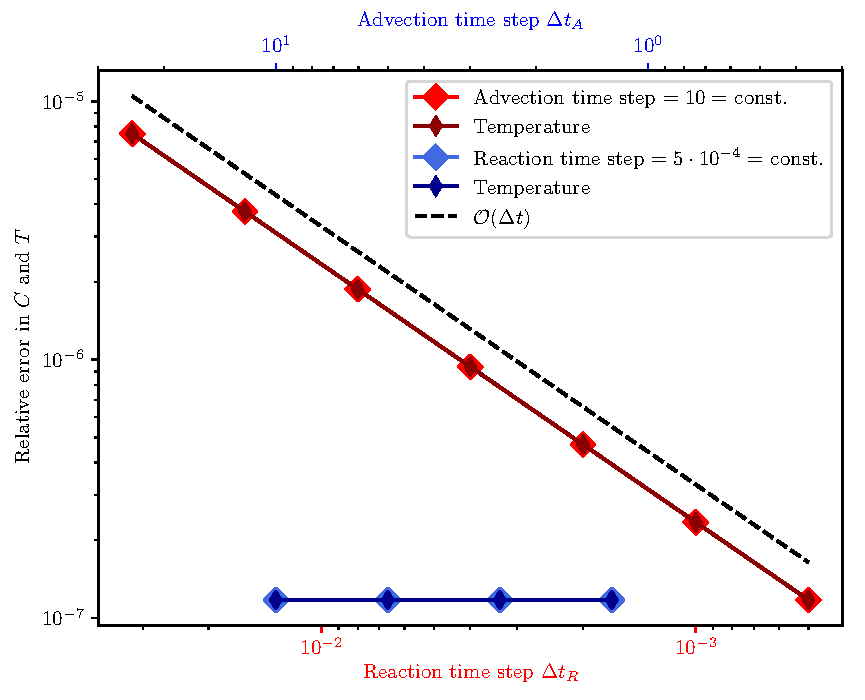
\includegraphics[width=0.65\textwidth]{cookbooks/benchmarks/operator_splitting/doc/error_exponential_decay.pdf}
  \end{center}
  \caption{\it Error for both compositional field and temperature compared to the analytical solution, varying the time steps of advection (blue data points and and top/blue x axis) and reactions (red data points and and bottom/red x axis), while keeping the other one constant, respectively.}
  \label{fig:exponential-decay}
\end{figure}

For the second benchmark case, we want to see the effect of advection on convergence.
In order to do this, we choose an initial temperature and composition that depends on x (in this case a sine), a decay rate that linearly depends on z, and we apply a constant velocity in x-direction on all boundaries. Our new analytical solution for the evolution of composition is now
 \begin{align}
  \mathfrak{c}(t)
  &=
  \sin (2\pi(x-t v_0)) \, \mathfrak{c}_0 e^{\lambda z t}.
\end{align}
$v_0$ is the constant velocity, which we set to 0.01 m/s.
The parameter file for this setup can be found in \url{benchmarks/operator_splitting/advection_reaction/advection_reaction.base.prm}.
\begin{figure}
  \begin{center}
    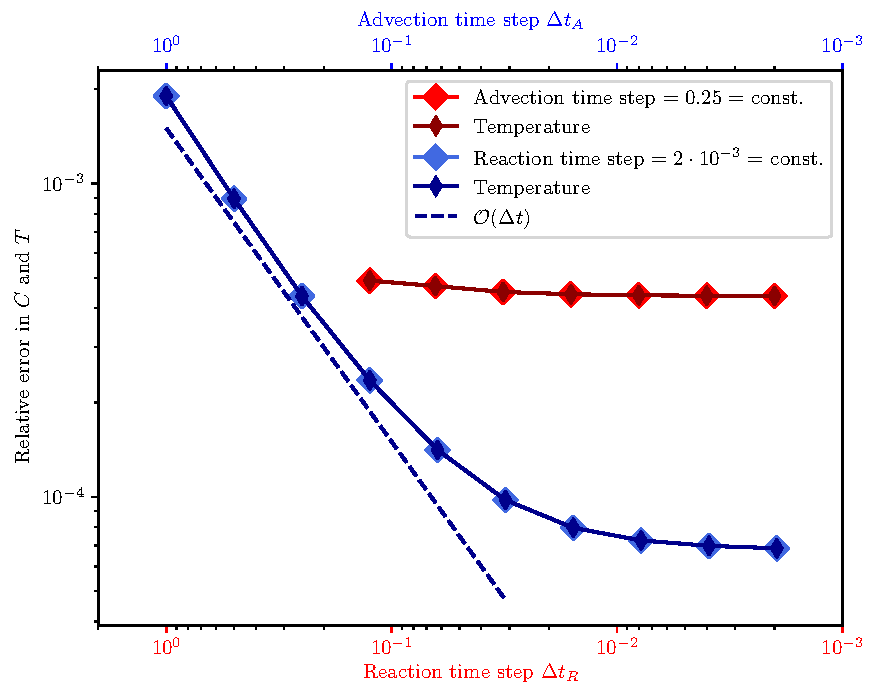
\includegraphics[width=0.48\textwidth]{cookbooks/benchmarks/operator_splitting/doc/error_advection_reaction.pdf}
    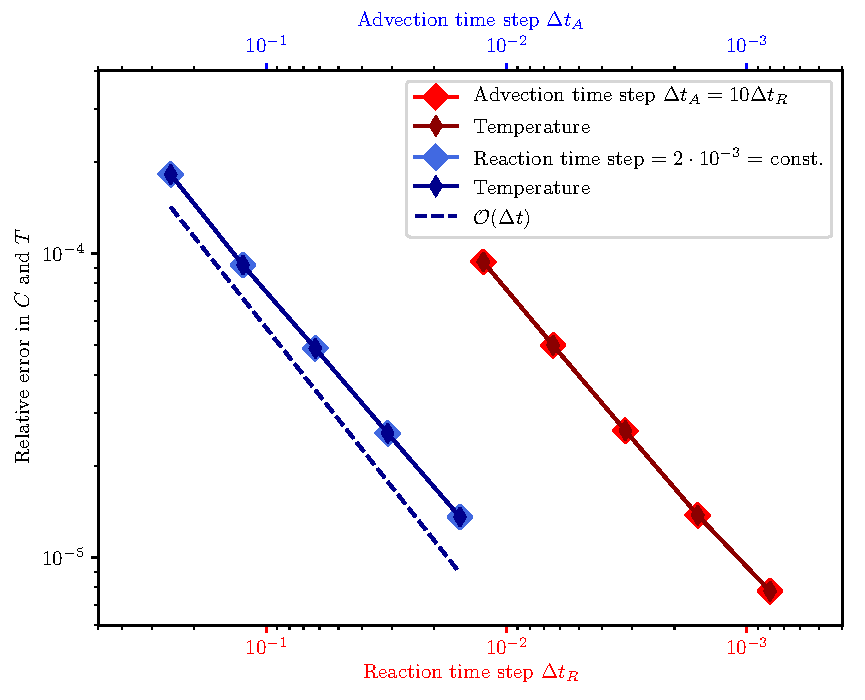
\includegraphics[width=0.48\textwidth]{cookbooks/benchmarks/operator_splitting/doc/error_advection_reaction2.pdf}
  \end{center}
  \caption{\it Error for both compositional field and temperature compared to the analytical solution, varying the time steps of advection (blue data points and and top/blue x axis) and reactions (red data points and and bottom/red x axis), while keeping the other one constant, respectively.}
  \label{fig:advection-reaction}
\end{figure}
Figure~\ref{fig:advection-reaction} shows the convergence behavior in this second set of models:
If we choose the same resolution as in the previous example (left panel), for large advection time steps $\Delta t_A > 0.1$ the error is dominated by advection, and converges with decreasing advection time step size (blue data points). However, for smaller advection time steps, the error stagnates. The data series where the reaction time step varies also shows a stagnating error. The reason for that is probably that our analytical solution is not in the finite element space we chose, and so neither decreasing the advection or the reaction time step will improve the error.
If we increase the resolution by a factor of 4 (right panel), we see that that errors converge both with decreasing advection and reaction time steps.

The results shown here can be reproduced using the bash scripts \texttt{run.sh} in the corresponding benchmark folders.
